\section{量子回路}
\label{sec:quantum-circuits}
% Reusable circuit symbols for the tables in Section 2.4.
% All wires run from left to right; for multi-qubit gates the upper wire
% is the leftmost tensor factor.
\tikzset{
  gatetablewire/.style={line width=0.7pt},
  gatetablebox/.style={draw,fill=white,line width=0.7pt,
    minimum width=0.62cm,minimum height=0.56cm,inner sep=1pt}
}

\newcommand{\GateTableSingle}[1]{%
  \begin{tikzpicture}[baseline=(current bounding box.center)]
    \draw[gatetablewire] (0,0) -- (2.4,0);
    \node[gatetablebox] at (1.2,0) {$#1$};
  \end{tikzpicture}%
}

\newcommand{\GateTableControlled}[1]{%
  \begin{tikzpicture}[baseline=(current bounding box.center)]
    \path[use as bounding box] (0,-0.90) rectangle (2.4,0.90);
    \draw[gatetablewire] (0,0.42) -- (2.4,0.42);
    \draw[gatetablewire] (0,-0.42) -- (2.4,-0.42);
    \draw[gatetablewire] (1.2,-0.42) -- (1.2,0.42);
    \fill (1.2,0.42) circle (1.8pt);
    \node[gatetablebox] at (1.2,-0.42) {$#1$};
  \end{tikzpicture}%
}

\newcommand{\GateTableCNOT}{%
  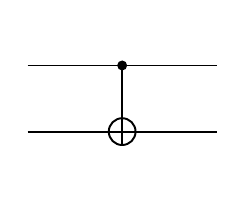
\begin{tikzpicture}[baseline=(current bounding box.center)]
    \path[use as bounding box] (0,-0.90) rectangle (2.4,0.90);
    \draw[gatetablewire] (0,0.42) -- (2.4,0.42);
    \draw[gatetablewire] (0,-0.42) -- (2.4,-0.42);
    \draw[gatetablewire] (1.2,-0.42) -- (1.2,0.42);
    \fill (1.2,0.42) circle (1.8pt);
    \draw[gatetablewire,fill=white] (1.2,-0.42) circle (0.17);
    \draw[gatetablewire] (1.04,-0.42) -- (1.36,-0.42);
    \draw[gatetablewire] (1.2,-0.58) -- (1.2,-0.26);
  \end{tikzpicture}%
}

\newcommand{\GateTableSWAP}{%
  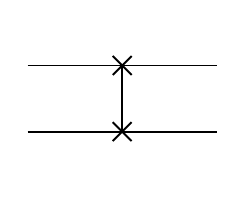
\begin{tikzpicture}[baseline=(current bounding box.center)]
    \path[use as bounding box] (0,-0.90) rectangle (2.4,0.90);
    \draw[gatetablewire] (0,0.42) -- (2.4,0.42);
    \draw[gatetablewire] (0,-0.42) -- (2.4,-0.42);
    \draw[gatetablewire] (1.2,-0.42) -- (1.2,0.42);
    \foreach \y in {0.42,-0.42} {
      \draw[gatetablewire] (1.08,\y-0.12) -- (1.32,\y+0.12);
      \draw[gatetablewire] (1.08,\y+0.12) -- (1.32,\y-0.12);
    }
  \end{tikzpicture}%
}

\newcommand{\GateTableToffoli}{%
  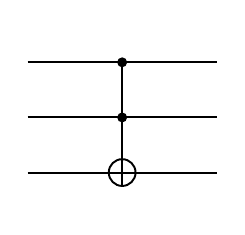
\begin{tikzpicture}[baseline=(current bounding box.center)]
    \path[use as bounding box] (0,-1.14) rectangle (2.4,1.14);
    \foreach \y in {0.70,0,-0.70} {
      \draw[gatetablewire] (0,\y) -- (2.4,\y);
    }
    \draw[gatetablewire] (1.2,-0.70) -- (1.2,0.70);
    \fill (1.2,0.70) circle (1.8pt);
    \fill (1.2,0) circle (1.8pt);
    \draw[gatetablewire,fill=white] (1.2,-0.70) circle (0.17);
    \draw[gatetablewire] (1.04,-0.70) -- (1.36,-0.70);
    \draw[gatetablewire] (1.2,-0.86) -- (1.2,-0.54);
  \end{tikzpicture}%
}


\subsection{量子回路の書き方}

古典コンピュータの計算は，論理ゲートを組み合わせた回路として表せる．
量子コンピュータでも同様に，量子ゲートを用いた量子回路として計算を表すことができる．
回路の横線は量子ビットを表し，左から右へ向かう順にゲートが作用する．

図\ref{fig:three-qubit-circuit-example}は，３量子ビットに操作する量子回路である．
図の右端の計器を描いた箱は計算基底での測定を表す．
\begin{figure}[H]
    \centering
    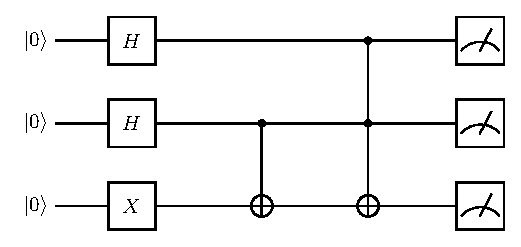
\includegraphics[width=0.76\textwidth]{figures/02-quantum-basics/three-qubit-circuit-example.pdf}
    \caption{３量子ビットに操作する量子回路の例}
    \label{fig:three-qubit-circuit-example}
\end{figure}
\newpage

\subsection{1量子ビットの量子回路}

代表的な1量子ビットゲートを表\ref{tab:single-qubit-gates}に示す．
行列表記は計算基底$\{\ket{0},\ket{1}\}$に関するものである．

\begin{table}[H]
    \centering
    \caption{代表的な1量子ビットゲート}
    \label{tab:single-qubit-gates}
    \footnotesize
    \renewcommand{\arraystretch}{1.35}
    \newcommand{\GateTableMatrix}[1]{\raisebox{0pt}[\dimexpr\height+2pt\relax][\dimexpr\depth+2pt\relax]{$#1$}}
    \begin{tabular}{|>{\centering\arraybackslash}m{17mm}|>{\raggedright\arraybackslash}m{39mm}|>{\centering\arraybackslash}m{32mm}|>{\centering\arraybackslash}m{54mm}|}
        \hline
        名前            & 意味                           & 回路                            & 行列表記                                                                                        \\ \hline
        $X$ゲート        & $X$軸周りに反転する                  & \GateTableSingle{X}           & \GateTableMatrix{\begin{bmatrix}0&1\\1&0\end{bmatrix}}                                                      \\ \hline
        $Y$ゲート        & $Y$軸周りに反転する                  & \GateTableSingle{Y}           & \GateTableMatrix{\begin{bmatrix}0&-\mathrm{i}\\\mathrm{i}&0\end{bmatrix}}                                   \\ \hline
        $Z$ゲート        & $Z$軸周りに反転する                  & \GateTableSingle{Z}           & \GateTableMatrix{\begin{bmatrix}1&0\\0&-1\end{bmatrix}}                                                     \\ \hline
        $H$ゲート        & $\ket{0}$と$\ket{1}$の重ね合わせを作る & \GateTableSingle{H}           & \GateTableMatrix{\dfrac{1}{\sqrt{2}}\begin{bmatrix}1&1\\1&-1\end{bmatrix}}                                  \\ \hline
        $S$ゲート        & Z軸周りに$\pi/2$回転する             & \GateTableSingle{S}           & \GateTableMatrix{\begin{bmatrix}1&0\\0&\mathrm{i}\end{bmatrix}}                                             \\ \hline
        $T$ゲート        & Z軸周りに$\pi/4$回転する             & \GateTableSingle{T}           & \GateTableMatrix{\begin{bmatrix}1&0\\0&e^{\mathrm{i}\pi/4}\end{bmatrix}}                         \\ \hline
        $R_x(\theta)$ & $X$軸周りに$\theta$回転する          & \GateTableSingle{R_x(\theta)} & \GateTableMatrix{\begin{bmatrix}\cos\frac{\theta}{2}&-\mathrm{i}\sin\frac{\theta}{2}\\-\mathrm{i}\sin\frac{\theta}{2}&\cos\frac{\theta}{2}\end{bmatrix}} \\ \hline
        $R_y(\theta)$ & $Y$軸周りに$\theta$回転する          & \GateTableSingle{R_y(\theta)} & \GateTableMatrix{\begin{bmatrix}\cos\frac{\theta}{2}&-\sin\frac{\theta}{2}\\\sin\frac{\theta}{2}&\cos\frac{\theta}{2}\end{bmatrix}} \\ \hline
        $R_z(\theta)$ & $Z$軸周りに$\theta$回転する          & \GateTableSingle{R_z(\theta)} & \GateTableMatrix{\begin{bmatrix}e^{-\mathrm{i}\theta/2}&0\\0&e^{\mathrm{i}\theta/2}\end{bmatrix}} \\ \hline
    \end{tabular}
\end{table}

\subsection{特別な記法のある量子回路}

制御ゲートやSWAPゲートなど，複数量子ビットに作用するゲートには特別な回路記号が用いられる．
複数量子ビットに作用する代表的なゲートを表\ref{tab:special-circuit-gates}に示す．
制御ゲートの黒丸は制御量子ビットを表し，$\ket{1}$のときにターゲット量子ビットへの演算が作用する．

\begin{table}[H]
    \centering
    \caption{特別な回路記号を用いるゲート}
    \label{tab:special-circuit-gates}
    \footnotesize
    \renewcommand{\arraystretch}{1.25}
    \begin{tabular}{|>{\centering\arraybackslash}m{20mm}|>{\raggedright\arraybackslash}m{40mm}|>{\centering\arraybackslash}m{31mm}|>{\centering\arraybackslash}m{51mm}|}
        \hline
        名前              & 意味                               & 回路                      & ディラック表記                                                                                               \\ \hline
        制御$U$           & 上の量子ビットが$\ket{1}$のとき，下に$U$を作用させる & \GateTableControlled{U} & $\ket{0}\bra{0}\otimes I+\ket{1}\bra{1}\otimes U$                                                     \\ \hline
        CNOT            & 上が$\ket{1}$のとき，下の量子ビットを反転する      & \GateTableCNOT          & $\ket{0}\bra{0}\otimes I+\ket{1}\bra{1}\otimes X$                                                     \\ \hline
        制御$Z$           & 両方が$\ket{1}$の成分の符号を反転する          & \GateTableControlled{Z} & $\ket{0}\bra{0}\otimes I+\ket{1}\bra{1}\otimes Z$                                                     \\ \hline
        SWAP            & 二つの量子ビットの状態を交換する                 & \GateTableSWAP          & $\ket{00}\bra{00}+\ket{10}\bra{01}+\ket{01}\bra{10}+\ket{11}\bra{11}$                                 \\ \hline
        Toffoli (CCNOT) & 上の2量子ビットがともに$\ket{1}$のとき，下を反転する  & \GateTableToffoli       & $\bigl(\ket{00}\bra{00}+\ket{01}\bra{01}+\ket{10}\bra{10}\bigr)\otimes I + \ket{11}\bra{11}\otimes X$ \\ \hline
    \end{tabular}
\end{table}

\subsection{量子回路の計算}
例として，図\ref{fig:three-qubit-circuit-example}の回路を考える．
初期の量子状態は$\ket{000}$であり，第１量子ビットと第２量子ビットに$H$ゲートを作用させ，下段に$X$ゲートを作用させる．
\begin{align*}
    \left(H \otimes H \otimes X\right)\ket{000}
     & = \frac{1}{\sqrt{2}}(\ket{0}+\ket{1}) \otimes \frac{1}{\sqrt{2}}(\ket{0}+\ket{1}) \otimes \ket{1} \\
     & = \frac{1}{2}\ket{001} + \frac{1}{2}\ket{011} + \frac{1}{2}\ket{101} + \frac{1}{2}\ket{111}
\end{align*}
次に，第２量子ビットを制御ビットとするCNOTゲートを第３量子ビットに作用させる．
第２量子ビットが$1$である項の第３量子ビットが反転する．
\begin{align*}
     & \left(I \otimes \left( \ket{0}\bra{0} \otimes I + \ket{1}\bra{1} \otimes X \right)\right)
    \left(\frac{1}{2}\ket{001} + \frac{1}{2}\ket{011} + \frac{1}{2}\ket{101} + \frac{1}{2}\ket{111}\right) \\
     & \quad= \frac{1}{2}\ket{001} + \frac{1}{2}\ket{010} + \frac{1}{2}\ket{101} + \frac{1}{2}\ket{110}
\end{align*}
最後に，第１量子ビットと第２量子ビットを制御ビットとするToffoliゲートを第３量子ビットに作用させる．
第１量子ビットと第２量子ビットがともに$1$である項の第３量子ビットが反転する．
\begin{align*}
     & \left(\left( \ket{00}\bra{00}+\ket{01}\bra{01}+\ket{10}\bra{10}\right)\otimes I + \ket{11}\bra{11}\otimes X\right)
    \left(\frac{1}{2}\ket{001} + \frac{1}{2}\ket{010} + \frac{1}{2}\ket{101} + \frac{1}{2}\ket{110}\right)                \\
     & \quad= \frac{1}{2}\ket{001} + \frac{1}{2}\ket{010} + \frac{1}{2}\ket{101} + \frac{1}{2}\ket{111}
\end{align*}
測定すると，$\left(\dfrac{1}{2}\right)^2 = \dfrac{1}{4}$の確率で$\ket{001}$，$\ket{010}$，$\ket{101}$，$\ket{111}$の各状態が得られる．
